% ============================================================================
% \sysname preprint (arxiv style, pdflatex)
%
% HONESTY DISCIPLINE (the paper's signature): every mechanism claim carries a
% status tag (three macros below). USE THEM on every claim; no over-claiming.
%   \statusdesign   -> design fully specified & documented, not yet coded
%   \statusmech     -> code implemented, unit-tested, mechanism in place
%   \statusdeferred -> end-to-end empirical validation deferred (state why)
%
% TERMINOLOGY DECOUPLING (hard constraint, from patent FTO discipline):
%   FORBIDDEN in body text: curvature / holonomy / fibre bundle / fiber bundle
%   USE INSTEAD: loop-closure defect / cycle-inconsistency / integer graph
%   (academic terms allowed only in Related Work when citing prior literature.)
%
% FOUR RED-LINE TRAPS (must carry a footnote/qualifier every time they appear):
%   G1 conversation / fluent dialogue  -> currently word/phrase-level only
%   G2 "achieved weaning"              -> statistical_weaning_ready != can_ween; can_ween permanently False
%   G3 coherent-sentence generation    -> deferred on perf wall
%   G4 language-domain weaning         -> can_ween(language) permanently False (accepted)
% ============================================================================
\documentclass[11pt,a4paper]{article}

\usepackage[utf8]{inputenc}
\usepackage[T1]{fontenc}
\usepackage{lmodern}
\usepackage{amsmath,amssymb,amsthm}
\usepackage{mathtools}
\usepackage{graphicx}
\usepackage{booktabs}
\usepackage{longtable}
\usepackage{array}
\usepackage{enumitem}
\usepackage{microtype}
\usepackage{xcolor}
\usepackage{algorithm,algpseudocode}
\usepackage{tikz}
\usetikzlibrary{arrows.meta, positioning, fit, calc, shapes.geometric}
\usepackage[colorlinks=true,linkcolor=blue,citecolor=blue,urlcolor=blue]{hyperref}
\usepackage{geometry}
\geometry{margin=1in}
\usepackage{natbib}
\usepackage{titlesec}

% ---- Honesty status tags (signature device of this paper) -----------------
\newcommand{\statusdesign}{\textcolor{purple}{\small\textsf{[design-complete]}}}
\newcommand{\statusmech}{\textcolor{teal}{\small\textsf{[mechanism-in-place]}}}
\newcommand{\statusdeferred}{\textcolor{orange}{\small\textsf{[end-to-end deferred]}}}
% Example: ``The system learns correspondences by tally-to-promote \statusmech.''

% ---- Footnote boilerplate (reuse project's own footnote discipline) -------
\newcommand{\footnotewall}{\footnote{This capability dimension collides with a
  definitive truth/grounding wall (\#479) that float-based systems also cannot
  cross; it is not a unique failure of this architecture.}}
\newcommand{\footnoteweaning}{\footnote{Statistical-weaning readiness
  (\textit{statistical\_weaning\_ready}) is defined to be strictly weaker than
  truth-valued weaning (\textit{can\_ween}); the latter is permanently False
  for the language domain by design (accepted, non-blocking).}}
\newcommand{\footnotestable}{\footnote{Stable output $\neq$ semantically
  correct: anti-theater testing validates that the \emph{criterion} is
  falsifiable, not that the system is semantically correct.}}

% ---- Theorem-like environments -------------------------------------------
\newtheorem{invariant}{Invariant}
\newtheorem{property}{Property}
\newtheorem{definition}{Definition}

% ---- System name macro ----------------------------------------------------
% Display name for the preprint. The implementation package is
% pure_integer_ai (named for its core invariant, not a trademark); PIDSLCA
% is the presentation name used throughout this paper.
\newcommand{\sysname}{PIDSLCA}

% ---- Title block ----------------------------------------------------------
\title{Exploring an Intelligent System Built Entirely on Integers\\
       \large \sysname{} --- A Pure-Integer Self-Learning Architecture
       with Interlocking Invariants}
\author{Jing Jianbin}
\date{\today}

\begin{document}
\maketitle

% ============================================================================
\begin{abstract}
We ask whether an intelligent system can be built entirely on
integers---not as a fixed-point substitute for floats, but as a
discrete, addressable, and auditable representation of learned facts,
so that learning is the reinforcement of those structures rather than
the adjustment of continuous weights. We present \sysname, a system
whose core is held together by six interlocking invariants that ensure
storage, addressing, matching, inference, and verification are
pure-integer operations, yielding bit-identical reproducibility. We
report one domain, arithmetic, in which the construction runs end to
end: the system compiles a symbolic specification, executes it on an
integer virtual machine, self-checks the result by recomputation, and
passes a six-gate readiness check we define narrowly and falsifiably.

We state the scope plainly. The arithmetic result is a mechanism
demonstration on a small, hand-shaped corpus---template abstraction, not
acquired arithmetic in any strong sense. We explicitly do not claim
competent language generation or truth-valued weaning: the language
domain is under active construction and is currently held back by an
engineering (performance) wall, not an architectural one. Every
mechanism claim carries one of three status tags---\textit{design-complete},
\textit{mechanism-in-place}, \textit{end-to-end-deferred}---so that no
mechanism is over-claimed.

\medskip\noindent\textbf{Keywords:} integer-represented intelligent
system; pure-integer learning; bit-level reproducibility; interlocking
invariants; statistical weaning; anti-theater discipline.
\end{abstract}

% ============================================================================
\section{Introduction}
\label{sec:intro}

% --------------------------- Motivation ------------------------------------
\subsection{Our Starting Point}
\label{sec:intro-start}

This work did not begin as a research programme. It began with an
irritation familiar to anyone who uses AI assistants: they forget. Each
conversation starts from nothing; what was picked up in one session does
not carry to the next. And for someone whose own machine cannot run a
large language model locally, the assistant and its forgetting live
together in the cloud, out of reach. The first thought behind this
project was plain: if the things a system learns were stored locally and
treated as memory, remembering would hang on durable storage that
survives between sessions, not on a context window that empties.

That thought raised the one that led to integers. If memory and learning
were to live in local storage rather than in a weight matrix trained on a
GPU, what is the least representation that could carry them? The guess
that started the construction was that integers might be enough; a
second half of the same guess---that they might also cost less than the
floating-point arithmetic that drives large models---turned out to be
wrong, and we record that in Section~\ref{sec:lim-perf} rather than
retcon a cleaner origin. What survived was the other half. Once learned
state was represented as integer structures, each learned fact became a
discrete, addressable thing: a person can point to the edge that carries
it, watch it strengthen as evidence accumulates, and tell it apart from
one the teacher supplied. Each change is auditable one fact at a time,
and because integer arithmetic is exact and associative, behaviour
reproduces across machines without the noise that continuous
representations drag along. The question this paper pursues grew out of
that, not out of the cost hope: \emph{can the whole of what a system
learns be carried by integer structures alone?}---not floating-point
stored differently, but discrete, exact, addressable facts, so that to
learn is to strengthen an edge rather than to nudge a coefficient.

We do not assume the answer is yes. The rest of the paper reports how
far the construction goes: what keeps it pure-integer, the constraints
it had to keep for the construction not to collapse on itself, and one
domain---a small one, whose scope we state in the open---in which the
approach runs end to end, alongside a second domain still under
construction where we report the terrain as it is.

\subsection{Motivation}
\label{sec:intro-motivation}

Float-based learning systems---large language models, graph neural
networks, reinforcement learners---share three internal defects that we
argue are not engineering accidents but consequences of representing
learned state as floating-point numbers.

\begin{enumerate}[leftmargin=*]
\item \textbf{Non-associativity undermines reproducibility.} Floating-point
addition is not associative: $(a+b)+c \neq a+(b+c)$ in general. The final
sum depends on evaluation order, which depends on hardware, BLAS kernel
selection, parallel reduction tree, and runtime version. The same trained
model therefore produces different outputs across machines, and even
across runs on the same machine when nondeterministic kernels are
involved. Strict A/B comparison---the bedrock of scientific evaluation of
a learning system---is consequently unattainable in principle, not merely
in practice.

\item \textbf{The learned state is opaque to audit.} A real-valued weight
matrix admits no human-readable decomposition into discrete learned
facts. One cannot point to ``the edge that says cats are animals'' as a
distinguished datum; the fact is smeared across thousands of coefficients.
Learning becomes a black box not by intent but by representation.

\item \textbf{Teacher boundaries are blurred.} In float systems the
external training signal (loss gradients) and the system's internal state
occupy the same continuous space; there is no structural seam between
``what the teacher injected'' and ``what the system learned on its own.''
Claims of self-learning become correspondingly hard to verify.
\end{enumerate}

\sysname is our attempt to show that a non-trivial self-learning system
can be built on a representation---the integer---that removes all three
defects by construction: integer arithmetic is associative and exact;
integer edges are individually addressable and auditable; and the teacher
can be structurally confined to a disjoint
companion store.

\subsection{Contributions}
\label{sec:intro-contrib}

\begin{itemize}[leftmargin=*]
\item \textbf{C1.} The construction of an intelligent-system core that is
strictly pure-integer---storage, addressing, matching, inference, and
verification contain no floating-point arithmetic---and that runs, showing
such a system can be built at all \statusmech.
\item \textbf{C2.} The six interlocking invariants that hold the
construction together, each backed by a mechanical check, with the
dependency structure among them stated explicitly rather than waved
through \statusmech.
\item \textbf{C3.} Bit-identical cross-hardware reproducibility as a
consequence of C1--C2: under a fixed gate configuration the same input
yields identical output bytes, giving strict A/B comparability that
continuous-representation systems cannot match \statusmech.
\item \textbf{C4.} One domain in which the construction runs end to
end---arithmetic---together with a narrow, falsifiable six-gate
readiness check. We are precise about the scope: this is a mechanism
demonstration on a small, hand-shaped corpus, not acquired arithmetic in
any strong sense, and the limitation is stated in the body, not buried
in a footnote \statusmech.
\end{itemize}

The construction is held to its claims by an anti-theater practice
(stable $\neq$ correct; every mechanism must have a live consumer and a
falsifiable test), which we describe in Section~\ref{sec:antitheater} as
the supporting discipline that keeps the exploration honest rather than
as a result in itself.

We deliberately do \emph{not} claim: fluent dialogue, truth-valued
weaning, coherent end-to-end sentence generation, or multimodal
capability. The honest scope of each mechanism is given in
Section~\ref{sec:limitations}.

% --------------------------- Design Principles -----------------------------
\subsection{Our Design Principles}
\label{sec:intro-principles}

Behind the mechanisms in later sections is a small set of design choices
that we state up front, because they are the points a reader is most
likely to question. Each is a stance about what learning and knowledge
\emph{are} in such a system, and each is defended in detail where the
relevant mechanism is presented; we state them here only as signposts.

Learning is the reinforcement of discrete structure, not the adjustment
of weights (Section~\ref{sec:arch-learning}). What the teacher supplied
and what the system learned must be separable, on pain of being unable to
tell them apart (Invariant I5; Section~\ref{sec:arch-storage}). Readiness
is not a single bit but a decomposable, falsifiable verdict
(Section~\ref{sec:antitheater}). And stable output is not correctness: a
mechanism that passes its tests may still be wired to pass regardless of
whether it learned anything, which is why every mechanism is held to a
live consumer and a falsifiable test (Section~\ref{sec:antitheater}).

% --------------------------- Roadmap ---------------------------------------
\subsection{Roadmap}
\label{sec:intro-roadmap}
Section~\ref{sec:arch} constructs the pure-integer system and states the
two-strata design stance. Section~\ref{sec:invariants} states the six
invariants that keep the construction from collapsing.
Section~\ref{sec:bitidentical} presents bit-identical reproducibility as
the supporting property that makes the exploration auditable.
Section~\ref{sec:mechanisms} surveys mechanisms, taking the arithmetic
domain first as an end-to-end demonstration whose small scope we state
plainly, each tagged with its status.
Section~\ref{sec:antitheater} sets out the anti-theater practice that
keeps the exploration honest. Section~\ref{sec:limitations} reports the
language-domain terrain honestly. Section~\ref{sec:related} discusses
related work.
Section~\ref{sec:conclusion} concludes.

% ============================================================================
\section{Construction of the Pure-Integer System}
\label{sec:arch}

\subsection{What We Represent: Two Strata of Logic}
\label{sec:arch-strata}

Before the layers, we state a design stance that shapes them. The
knowledge such a system carries is not one uniform kind of relation but
two, with different mathematical groundings, and we represent them with
different kinds of integer edge because they admit different operations.
Conflating the two is a recurring source of error, so we keep them
explicit.

The first stratum is \emph{structural} logic---the logic of ``what kind
of thing this is.'' Class inclusion (an \texttt{IS\_A} edge: a cat is an
animal), equivalence (a \texttt{PURE\_ALIAS} edge: an apple is an
\textit{apple} in another language), and part-whole composition
(\texttt{MEREOLOGY}) answer questions of category and identity. These
are set-theoretic relations; their natural operation is closure---the
transitive closure of inclusion (the ancestor class of a concept), the
equivalence class of an alias---computed once and used to constrain what
may fill a slot or to recognise a category.

The second stratum is \emph{causal and temporal} logic---the logic of
``what leads to what.'' Sequential precedence (\texttt{PRECEDES}: one
token before another), causation (\texttt{CAUSES}: one event bringing
about another), and ordered composition (\texttt{COMPOSES}: parts
assembled in an order) answer questions of dependence. These are
order-theoretic relations; their natural operation is the partial
order---topological layering and reachability along a directed acyclic
graph---which we use to drive generation step by step. The
downward-only dependency invariant (I6) is itself an instance of this
stratum: the layer graph is a DAG, and an upper layer may depend on a
lower one but never back.

This split is a design choice, not an after-the-fact taxonomy. The two
strata misbehave under each other's operations: taking the closure of a
causal edge as if it were set inclusion blurs cause into class; taking
the topological order of an equivalence edge as if it were precedence
imposes a false direction on a symmetric fact. Representing both on one
integer graph---closure-bearing or symmetric edges for the structural
stratum, directed acyclic edges for the causal stratum, all on integer
endpoints with integer strength---is what lets a single representation
serve both without the operations of one corrupting the other.

Within the causal stratum, sequential order deserves a precise statement,
because it is where the representation does something learning does not.
A \texttt{PRECEDES} edge is written between consecutive tokens of a
sentence with constant strength; it is not promoted by co-occurrence
counting, and reward never adjusts it. Order is therefore a structural
constraint the representation honours, not a weight reinforcement
selects. The system is faithful to the order the corpus presents---a
sentence read as $(a,b,c)$ yields $a \to b \to c$---but it does not
statistically learn that order: it does not count which order is
frequent, and so does not on its own discover that an alternative order
(SOV where the corpus is SVO) is admissible. Encoding the order given,
rather than learning the admissibility of many orders, is the limit we
state here \statusmech.

\subsection{Layered Design}
\label{sec:arch-layers}

\sysname is organized into eight layers, $L_0$ (numeric foundation) at the
bottom through $L_7$ (edge adapters) at the top, with a strict
downward-only dependency discipline (Invariant I6): an upper layer may
import a lower one, never the reverse, and never laterally across the
core seam. The \emph{core}---layers $L_0$--$L_4$---is where all learned
state resides and where the six invariants hold absolutely. Layers
$L_5$--$L_7$ (teacher, evolution, edge) are the only layers permitted to
handle natural-language text, network I/O, and floating-point; they are
quarantined from the core by an import-direction test that verifies the
core never imports the edge. Table~\ref{tab:layers} summarizes the
responsibilities.

\begin{table}[t]
\centering
\small
\caption{Layer structure ($L_0$ foundation $\to$ $L_7$ edge). The core is
$L_0$--$L_4$; only $L_7$ handles text, network, and floating-point.}
\label{tab:layers}
\begin{tabular}{@{}p{0.08\linewidth}p{0.20\linewidth}p{0.64\linewidth}@{}}
\toprule
Layer & Name & Responsibility \\
\midrule
$L_0$ & Numeric      & Pure-integer foundation: bigint, algebraic fractions (exact long-division invariant), rational cross-product comparison, integer square root, int64 sparse matrix, golden hash, deterministic RNG, AST float guard. \\
$L_1$ & Storage      & Pure-integer tables (no float columns, no raw-text columns). \\
$L_2$ & Storage-VM   & Arithmetic virtual machine (sub/mul/mod operators). \\
$L_3$ & Calc         & Synthesis, capability store, sandbox. \\
$L_4$ & Cognition    & Graph topology, reasoning chains, Hebbian learning, structure discovery, activation. \\
$L_5$ & Teacher      & Define / reward / independent judge. \\
$L_6$ & Evolution    & Self-proof, emergence loop. \\
$L_7$ & Edge         & Text / network / LLM adapters; the sole float-bearing layer; companion-store quarantine. \\
\bottomrule
\end{tabular}
\end{table}

\subsection{Pure-Integer Storage and Companion Quarantine}
\label{sec:arch-storage}

\begin{figure}[t]
\centering
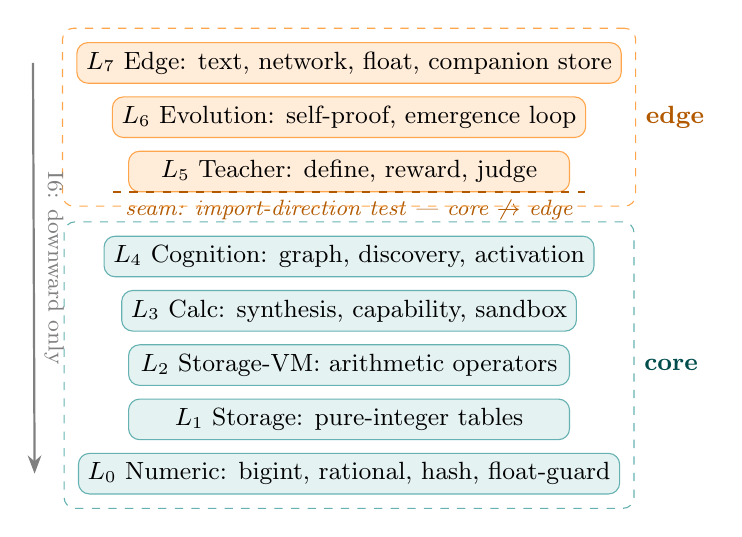
\begin{tikzpicture}[
  layer/.style={draw, rounded corners, minimum width=5.6cm, minimum height=0.5cm, font=\small},
  corelayer/.style={layer, fill=teal!10, draw=teal!60},
  edgelayer/.style={layer, fill=orange!15, draw=orange!70},
  node distance=0.16cm,
]
\node[edgelayer] (L7) {$L_7$ Edge: text, network, float, companion store};
\node[edgelayer, below=of L7] (L6) {$L_6$ Evolution: self-proof, emergence loop};
\node[edgelayer, below=of L6] (L5) {$L_5$ Teacher: define, reward, judge};
\node[corelayer, below=0.55cm of L5] (L4) {$L_4$ Cognition: graph, discovery, activation};
\node[corelayer, below=of L4] (L3) {$L_3$ Calc: synthesis, capability, sandbox};
\node[corelayer, below=of L3] (L2) {$L_2$ Storage-VM: arithmetic operators};
\node[corelayer, below=of L2] (L1) {$L_1$ Storage: pure-integer tables};
\node[corelayer, below=of L1] (L0) {$L_0$ Numeric: bigint, rational, hash, float-guard};
\draw[dashed, orange!70!black, thick] ([xshift=-3.0cm]L5.south) -- ([xshift=3.0cm]L5.south);
\node[font=\footnotesize\itshape, orange!70!black] at ([yshift=-0.22cm]L5.south) {seam: import-direction test --- core $\not\to$ edge};
\node[draw=orange!70, dashed, rounded corners, fit=(L5)(L6)(L7), inner sep=5pt] (edge) {};
\node[draw=teal!60, dashed, rounded corners, fit=(L0)(L1)(L2)(L3)(L4), inner sep=5pt] (core) {};
\node[font=\small\bfseries, orange!70!black, anchor=west] at (edge.east) {edge};
\node[font=\small\bfseries, teal!60!black, anchor=west] at (core.east) {core};
\draw[-Stealth, gray, thick] ([xshift=-0.55cm]L7.west) -- ([xshift=-0.55cm]L0.west) node[midway, sloped, above, font=\footnotesize]{I6: downward only};
\end{tikzpicture}
\caption{Layered architecture and the core/edge quarantine seam. The core
($L_0$--$L_4$, teal) holds all learned state under the six invariants and
never imports the edge; the edge ($L_5$--$L_7$, orange) is the sole
float- and text-bearing region, quarantined by an import-direction test
that verifies the core never imports the edge. Dependency is strictly
downward (Invariant I6).}
\label{fig:arch}
\end{figure}


A \emph{concept reference} is an integer pair
$(\textit{space\_id}, \textit{local\_id})$. Edges and attributes are
integer-typed throughout. The core storage at $L_1$ comprises a fixed set
of pure-integer tables; there are deliberately no floating-point columns
and no raw-text columns. Raw text and all teacher-injected material
reside in a disjoint \emph{companion store} at $L_7$, which the core never
imports. A source-disjoint assertion enforces the seam.

This quarantine is what makes the teacher-boundary invariant (I5)
mechanically enforceable rather than a matter of convention. Float-bearing
teacher content---for instance, real-valued word embeddings---cannot
reach the core because no import path exists across the seam. The
companion store admits only the narrow signal kinds permitted by I5
(name, define, reward, error-label), each written to a disjoint space.

\subsection{Learning as Edge-Count Reinforcement}
\label{sec:arch-learning}

Learning is not gradient descent. Edge strength is a monotonically
non-decreasing integer (Invariant I3); a relation is learned by the
repeated co-occurrence of its endpoints, which increments an integer
counter on the corresponding edge until the counter crosses a promotion
threshold---\emph{tally-to-promote}. There is no decay, no damping, and
no teleportation-style smoothing; an overwritten value leaves a trace in
the append-only audit (Invariant I4).

The training loop reads a corpus through the edge layer (tokenization,
then word-form-to-concept mapping via REFERS\_TO edges), activates
sentences in $L_4$, and applies Hebbian co-occurrence counting. Counting
is process-sharded into deterministic delta-plus-merge reductions so that
multi-core execution remains bit-identical (Invariant I2): the merge is a
sorted apply, independent of sharding order. Relations, function words,
and grammatical roles are themselves \emph{learned signals} rather than
hardcoded tables: a self-learning signal layer replaces any fixed
relation, function-word, or role lexicon, so the system acquires its
syntactic vocabulary from exposure rather than from a prespecified list
\statusmech.

Reward flows from the teacher layer ($L_5$) into reasoning-edge learning,
closing the loop
reward $\to$ strength $\to$ propagation-relevance $\to$ activation $\to$
generation.

\begin{algorithm}[t]
\caption{Tally-to-promote edge reinforcement}
\label{alg:tally}
\begin{algorithmic}[1]
\Require corpus $\mathcal{C}$, integer seed $s$, promotion threshold $\theta$
\Ensure learned edge set $E$ with integer strengths
\State seed the deterministic RNG with $s$; \ $E \gets \emptyset$
\For{each sentence $\sigma \in \mathcal{C}$, sharded deterministically}
  \For{each co-occurring concept pair $(u,v)$ in $\sigma$}
    \State $E[u,v].\textit{tally} \mathrel{+}{=} 1$ \Comment{monotone, I3}
  \EndFor
\EndFor
\State merge shards by sorted apply \Comment{order-independent $\Rightarrow$ bit-identical, I2}
\For{each $(u,v)$ with $E[u,v].\textit{tally} \geq \theta$}
  \State promote $E[u,v]$ to learned status
  \State append audit record \Comment{append-only, I4}
\EndFor
\State \textbf{return} $E$
\end{algorithmic}
\end{algorithm}

\subsection{Beyond Edge-Count: Other Acquisition and Check Means}
\label{sec:arch-learning-other}

Edge-count reinforcement is the learning primitive, but the system also
acquires and certifies structure by other integer operations, which we
name here only to mark their honest scope and then demonstrate where they
are shown. Structure is acquired by alignment---several samples sharing a
combinatorial shape are aligned position-by-position into a reusable
skeleton---which is template abstraction rather than algorithm discovery
(Section~\ref{sec:mech-discovery}). Relations the teacher asserts are
certified by a constructive self-check, not learned: the system executes
a declared composition and compares the result to identity, acquiring no
new edge beyond the rules it was given
(Section~\ref{sec:mech-inverse}). Sequential order, finally, is a
structural constraint of the causal stratum, not a learned strength
(Section~\ref{sec:arch-strata}). We defer the detail to those sections so
that ``learning'' is read as tally-to-promote alone, and so that the
things which are not learning are not smuggled in under that name.

\subsection{Memory: Reading and Interaction Layers}
\label{sec:arch-memory}

Memory is physically split into two layers. The \emph{reading layer}
($\textit{session\_id} = \textsc{null}$) holds consolidated experience
shared across sessions; the \emph{interaction layer} (per-session
$\textit{session\_id}$) holds ephemeral per-conversation state.
Post-weaning learning---the acquisition of new facts encountered during
interaction---is written to memory rather than to the core concept graph,
so that conversational acquisition does not pollute the trained core.
A memory item is promoted from experience to consolidated status by a
usage-ratio gate \statusmech. This split is what would later support an
online ``learn-by-asking'' capability without re-training; the
conversational shell itself is deferred \statusdeferred\ (see
Section~\ref{sec:limitations}).

% ============================================================================
\section{Six Interlocking Invariants}
\label{sec:invariants}

The pure-integer construction would be easy to undermine by quiet
exceptions---a little floating-point here, a little teacher injection
there---each harmless on its own. The six invariants below are the
constraints we found we had to keep for the construction not to collapse
on itself. They are not independent: each is enforced by a mechanical
check that depends on another, so the guarantees interlock. We state the
dependency structure explicitly, because it is weaker than the attractive
but false claim that the six form a single indivisible block.
Table~\ref{tab:invariants} states each invariant, its definition, and its
execution point (the mechanical check that enforces it).

\begin{table}[t]
\centering
\small
\caption{The six interlocking invariants, their definitions, and the
mechanical execution point that enforces each.}
\label{tab:invariants}
\begin{tabular}{@{}p{0.20\linewidth}p{0.40\linewidth}p{0.32\linewidth}@{}}
\toprule
Invariant & Definition & Execution point \\
\midrule
I1. Pure-integer &
Core storage, addressing, matching, inference, and verification contain
no floating-point arithmetic. Division uses an exact integer
\emph{long-division invariant}; comparison uses integer cross-products. &
Abstract-syntax-tree audit (CI, non-disableable) + runtime type probe. \\
\addlinespace
I2. Bit-identical reproducibility &
Same input and gate configuration yield bit-identical output across
hardware, OS, and build, verified by content hash. &
Reproducibility assertion + golden-snapshot tests. \\
\addlinespace
I3. Monotone-with-overwrite &
Edge strength is a monotonically non-decreasing integer; destructive
decay/damping/forgetting is out of scope; overwrites are traceable. &
Edge-strength monotonicity check in write path. \\
\addlinespace
I4. Append-only audit &
History records are append-only and tamper-evident; in-place destructive
updates fall outside the architecture. &
Append-only audit-event hash chain. \\
\addlinespace
I5. Teacher boundary &
External teacher supplies only name/define/reward/error labels into a
disjoint companion store; placement, order, punctuation, and co-occurrence
are never injected into the core. &
Source-disjoint assertion + teacher-boundary verifier. \\
\addlinespace
I6. Downward-only dependency &
The layer graph $L_0 \to L_1 \to \dots \to L_7$ is a DAG; upper layers
may import lower, never the reverse, never lateral across the core seam. &
Import-direction test. \\
\bottomrule
\end{tabular}
\end{table}

\subsection{Execution Points}
\label{sec:invariants-exec}

Each invariant is backed by a mechanical check rather than a convention.
The pure-integer invariant (I1) is enforced at two independent layers:
a static abstract-syntax-tree audit that rejects any floating-point
literal or operation in the core source, and a runtime probe
(\texttt{assert\_no\_float}) invoked at the entry of each numeric
component. The AST audit is non-disableable in continuous integration;
the runtime probe is disableable for debug but on by default. The
remaining invariants are enforced by the execution points listed in
Table~\ref{tab:invariants}.

A practical note on the long-term maintainability of this purity. The
failure mode a reader is right to worry about is a quietly imported
floating-point dependency---a C extension, a numerical library---that
the AST audit does not see. The current core forestalls this in the
narrow but checkable way available to a Python codebase: the core is
pure Python with no compiled C-extension dependency, so the surface across
which float could enter is the import graph the audit already walks, not
an un-audited native binary. The claim is therefore an engineering claim
about the present codebase (``no float enters the core today, and the path
that would let it enter is watched''), not a guarantee that the
architecture is immune to any future native dependency. Admitting such a
dependency would require widening the audit; we state this rather than
pretend the AST audit sees what it cannot \statusmech.

\subsection{Collapse under Relaxation}
\label{sec:invariants-collapse}

The necessity of each invariant is not aesthetic; it is load-bearing. We
state the concrete collapse that follows from relaxing each invariant in
turn, to make plain that no member can be quietly dropped.

\begin{itemize}[leftmargin=*]
\item \textbf{Relax I1 (admit float in the core).} Associativity is lost;
the merge order of sharded reductions now changes the result, so I2
collapses on the arithmetic side. Strict A/B comparison
(Section~\ref{sec:bitidentical}) becomes confounded with rounding noise.
\item \textbf{Relax I2 (drop the reproducibility assertion).} The system
may still run deterministically in principle, but a regression that
breaks determinism goes undetected; the auditable evolution of
Section~\ref{sec:antitheater} degrades from a checked property to trust.
\item \textbf{Relax I3 (admit decay or damping).} Edge strengths become
order-sensitive time series; the same corpus no longer yields the same
learned graph, so the determinism of the learned state is lost even with
integer arithmetic. The monotone ``learn or stay still'' semantics is lost.
\item \textbf{Relax I4 (admit in-place destructive update).} History
becomes mutable; a post-hoc edit to an edge can no longer be
distinguished from a genuine learning event, weakening the audits that
rely on a faithful history.
\item \textbf{Relax I5 (let the teacher write core state).} The seam
between teacher injection and self-learning is erased; a capability
observed at weaning can no longer be attributed to the system, so the
anti-theater discipline loses its falsifiable target.
\item \textbf{Relax I6 (admit lateral or upward import).} Float-bearing
edge code (text, network, real-valued embeddings) gains an import path
into the core, so I1 collapses by construction; the quarantine that
makes I1 and I5 mechanically enforceable is gone.
\end{itemize}

The architecture is therefore not a collection of best practices that
may be traded off independently: relaxing one invariant tends to collapse
the guarantee of another. We now state that interdependence precisely,
and honestly about where it does and does not bind.

\subsection{How the Invariants Underwrite One Another}
\label{sec:invariants-nonsep}

The six invariants are not independent conveniences; each is enforced by a
check that another invariant makes possible. Removing one does not merely
forfeit its own guarantee---it can collapse the guarantee of another:

\begin{itemize}[leftmargin=*]
\item \textbf{I2 depends on I1.} Bit-identical reproducibility is
unattainable the moment floating-point arithmetic enters the core, because
non-associative rounding makes output dependent on evaluation order.
\item \textbf{I3 depends on I4.} The traceability of a monotone overwrite
presupposes an append-only audit; without append-only history, an
overwrite erases the record of the prior value and the monotonicity
guarantee becomes unverifiable.
\item \textbf{I5 depends on I6.} The teacher can be confined to a disjoint
companion store only because the layer graph is acyclic and the core seam
is import-protected; a reverse or lateral dependency would let
teacher-injected material flow back into the core.
\item \textbf{I1 depends on I5.} The core remains pure-integer only because
the teacher cannot inject floating-point semantics (e.g., real-valued
embeddings) across the boundary; relaxing I5 admits float-bearing teacher
content into the core.
\end{itemize}

\noindent These four edges do \emph{not} form a single cycle. They
connect the six into two components: a four-chain
$I_6 \to I_5 \to I_1 \to I_2$ in which the teacher boundary, the
pure-integer core, and bit-identical reproducibility each prop up the
next, and a separate pair $I_4 \to I_3$ linking append-only audit to
monotone traceability. We state this plainly rather than claim the six
are indivisible: within the four-chain, removing any member breaks the
chain, but the pair $\{I_3, I_4\}$ can be lifted without toppling
$\{I_1, I_2, I_5, I_6\}$, and vice versa. What holds is the weaker,
honest claim---no invariant is an orphan (each has an underwriter), and
the four-chain is internally non-separable \statusmech.

\begin{figure}[t]
\centering
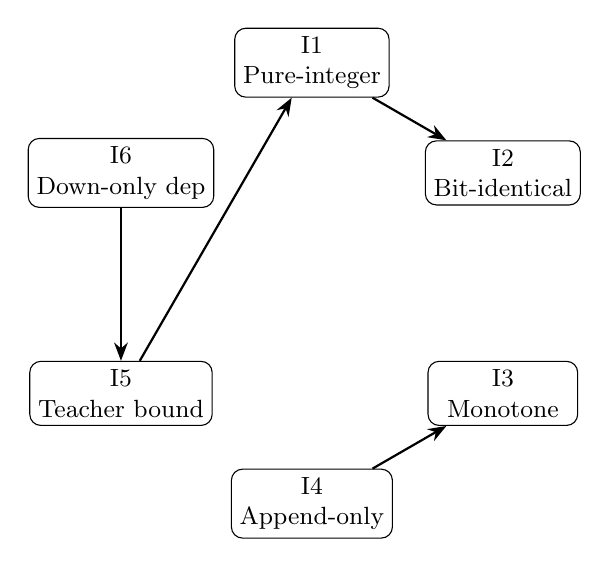
\begin{tikzpicture}[
  inv/.style={draw, rounded corners, minimum width=1.9cm, minimum height=0.7cm,
              font=\small, inner sep=3pt, align=center},
  >=Stealth]
\node[inv] (I1) at (90:2.8cm)   {I1\\Pure-integer};
\node[inv] (I2) at (30:2.8cm)   {I2\\Bit-identical};
\node[inv] (I3) at (-30:2.8cm)  {I3\\Monotone};
\node[inv] (I4) at (-90:2.8cm)  {I4\\Append-only};
\node[inv] (I5) at (-150:2.8cm) {I5\\Teacher bound};
\node[inv] (I6) at (150:2.8cm)  {I6\\Down-only dep};
\draw[->, thick] (I1) -- (I2);
\draw[->, thick] (I4) -- (I3);
\draw[->, thick] (I6) -- (I5);
\draw[->, thick] (I5) -- (I1);
\end{tikzpicture}
\caption{How the six invariants underwrite one another. An arrow
$X \to Y$ reads ``$X$ underwrites $Y$'': relaxing $X$ collapses the
guarantee of $Y$. The edges form two components: a four-chain
$I_6 \to I_5 \to I_1 \to I_2$ and a separate pair $I_4 \to I_3$. No
invariant is an orphan (each has an underwriter); the four-chain is
internally non-separable, but the pair and the chain can be lifted
independently, so we do not claim the six form a single indivisible
block.}
\label{fig:invariants}
\end{figure}

% ============================================================================
\section{Bit-Identical Cross-Hardware Reproducibility}
\label{sec:bitidentical}

\subsection{Reproducibility as a Derived Evaluation Property}
Bit-identical reproducibility is not a contribution standing on its own;
it is an evaluation property that follows from the invariants above.
Because the core satisfies the pure-integer invariant (I1) and the
deterministic-verification mechanisms (I2), two runs that claim to differ
only by an intended change can actually be checked to differ only by that
change---which is what makes the exploration auditable. As a technical
effect it follows from I1 combined with four mechanisms that jointly
eliminate every source of nondeterminism available to a Python program.
We describe each.

\subsection{The Deterministic Verification Family}

\paragraph{Append-only audit-event hash chain.}
Every state-mutating operation appends an audit event whose hash
incorporates the hash of the previous event (FNV-1a, 64-bit). The chain
is tamper-evident---any retroactive modification breaks it---and two
executions that perform the same operations produce identical chains,
yielding a verifiable fingerprint of the run.

\paragraph{Reproducibility assertion.}
A two-pass assertion runs the same computation under the same seed and
compares the terminal hash; equality is required. This converts
reproducibility from an empirical hope into a checked invariant.

\paragraph{Deterministic randomness source.}
The sole source of pseudo-randomness is a splitmix64-based deterministic
RNG. Nondeterministic sources---the \texttt{random} module, wall-clock
time, and \texttt{datetime}---are banned by the same AST audit that bans
floating-point. Randomness is therefore a pure function of an integer
seed.

\paragraph{Two-layer float guard.}
The pure-integer invariant (I1) is enforced at two independent layers: a
runtime probe, disableable for debugging, and a static AST audit that is
non-disableable in continuous integration. The AST audit is the
load-bearing layer; it cannot be silently turned off by a misconfigured
runtime, so the guarantee holds even when the runtime probe is off.

\subsection{Strict A/B Comparability}
The engineering value of bit-identical output is strict A/B
comparability: two configurations, two training runs, or two
architectural variants can be compared byte-for-byte, with any output
difference attributable solely to the intended change rather than to
nondeterministic noise. Float-based systems cannot offer this in
principle: non-associative rounding means that an identical configuration
produces different output across hardware, so A/B differences are
confounded with rounding noise and cannot be cleanly attributed to the
change under study.

\begin{figure}[t]
\centering
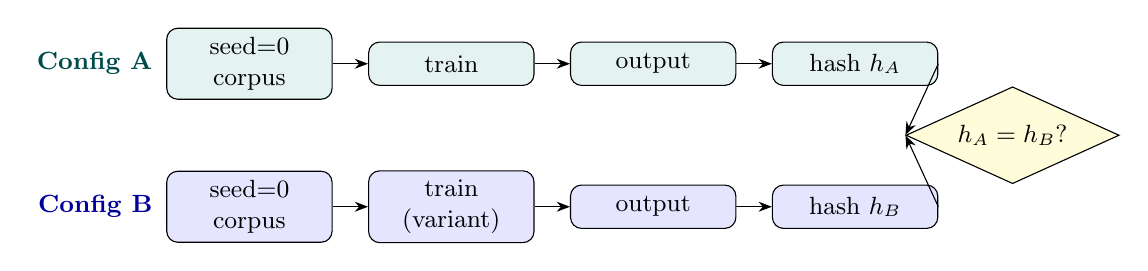
\begin{tikzpicture}[
  box/.style={draw, rounded corners, minimum width=2.1cm, minimum height=0.55cm, font=\small, align=center},
  abox/.style={box, fill=teal!10},
  bbox/.style={box, fill=blue!10},
  cmp/.style={draw, diamond, aspect=2.2, fill=yellow!15, font=\small, align=center, minimum width=1.6cm},
  node distance=0.45cm and 0.45cm,
]
\node[abox] (a1) {seed=0\\corpus};
\node[abox, right=of a1] (a2) {train};
\node[abox, right=of a2] (a3) {output};
\node[abox, right=of a3] (a4) {hash $h_A$};
\node[bbox, below=0.9cm of a1] (b1) {seed=0\\corpus};
\node[bbox, right=of b1] (b2) {train\\(variant)};
\node[bbox, right=of b2] (b3) {output};
\node[bbox, right=of b3] (b4) {hash $h_B$};
\draw[-Stealth] (a1) -- (a2); \draw[-Stealth] (a2) -- (a3); \draw[-Stealth] (a3) -- (a4);
\draw[-Stealth] (b1) -- (b2); \draw[-Stealth] (b2) -- (b3); \draw[-Stealth] (b3) -- (b4);
\node[cmp] at ($(a4)!0.5!(b4) + (2.0,0)$) (cmp) {$h_A = h_B$?};
\draw[-Stealth] (a4.east) -- (cmp.west);
\draw[-Stealth] (b4.east) -- (cmp.west);
\node[font=\small\bfseries, teal!60!black, left=0.05cm of a1] {Config A};
\node[font=\small\bfseries, blue!60!black, left=0.05cm of b1] {Config B};
\end{tikzpicture}
\caption{Strict A/B comparability. Two configurations run under the same
integer seed; their terminal hashes are compared byte-for-byte. Under a
fixed gate configuration the hashes match (bit-identical); any
difference is attributable solely to the intended change, never to
rounding noise---a property float-based systems cannot offer in
principle.}
\label{fig:ab}
\end{figure}

\subsection{Honest Scope}
The guarantee holds under a fixed gate configuration. New mechanisms are
admitted behind default-off gates
(Section~\ref{sec:antitheater}), so that the bit-identical baseline is
preserved; turning a gate on is an explicit, logged behavior change that
remains deterministic within the chosen configuration but is not
bit-identical to the gate-off baseline, by design. Exhaustive
cross-hardware measurement of the guarantee is \statusdeferred\
(mechanism in place; measurement across diverse hardware deferred to
future work).

% ============================================================================
\section{Mechanisms}
\label{sec:mechanisms}

The mechanisms below show what the system does. We take the arithmetic
domain first, because it is the one domain in which the construction
runs end to end on a real (if small) task, and we describe its scope at
length and in the open---it is smaller than a reader of the headline
might expect, and the temptation to overstate it is the temptation this
section exists to resist. The remaining mechanisms are surveyed more
briefly, each tagged with its status (\statusdesign/\statusmech/\statusdeferred).

\subsection{The Arithmetic Domain: An End-to-End Compiler Sanity Check}
\label{sec:mech-arith}

We prove the pipeline is complete. Given a symbolic arithmetic
specification supplied by the teacher, \sysname compiles it into an
integer \texttt{COMPOSES} graph, executes the graph on an integer
virtual machine using exact rational arithmetic, self-checks the result
by recomputation, and passes a six-gate readiness check that we define
narrowly and falsifiably. Compiler, virtual machine, self-check, and the
six gates all run, end to end, on the pure-integer core. That is the
demonstration this section reports, and the rest of it makes each step
and its scope concrete.

\subsubsection*{Compilation, not acquisition.}
The system is neither programmed with arithmetic in the ordinary sense
nor does it induce arithmetic from examples. A teacher supplies an
arithmetic specification in a deliberately small symbolic language
(addition, subtraction, multiplication, division, non-negative literal
powers, and bounded sum, product, and recurrence constructs). The system
parses that specification into a \texttt{COMPOSES} graph---integer nodes
for operands, operators, and control---and compiles the graph into
bytecode for an integer virtual machine. Execution uses exact integer
rational arithmetic (cross-product comparison, no floating point), so a
run is a deterministic, replayable computation rather than an
approximation. What the system does acquire on its own is structural: it
aligns several specifications that differ only in their parameter names,
extracts the shared parameterised skeleton, and reuses that skeleton on a
new parameter name or input value \statusmech. This is template
abstraction, not algorithm discovery, and we name it as such.

\subsubsection*{Self-check by recomputation.}
A generated answer is checked by executing the compiled graph a second
time and comparing. This closes a consistency loop inside the
architecture without crossing the truth/grounding wall, which forbids an
external oracle \statusmech. We are precise about what that loop does
and does not catch. Both executions derive from the same specification,
so the check is constructive: it catches compilation and execution
divergence, parameter misalignment, and non-determinism, but it cannot
catch a specification that is itself wrong, because both runs share the
error. It is an internal consistency check, not a test against ground
truth.

\subsubsection*{Cross-execution consistency.}
A second execution path is built by applying a restricted transformation
to the original specification, and agreement between the two paths is
taken as a stronger internal signal \statusmech. We record the limit
honestly: the two paths share a common origin, so a systematic error
present in both passes the check. The consistency signal is real but
single-sourced; a fully independent second builder is deferred
\statusdeferred.

\subsubsection*{A six-gate readiness check, on a toy corpus.}
The decisive question is whether the system keeps producing checked
answers once the teacher stops supplying specifications. We define
readiness as a six-gate verdict rather than a single bit, guarded by a
\emph{measured-guard} that vetoes a pass when the underlying measurement
is absent, so a silent or unmeasured system cannot pass by default
\statusmech\footnoteweaning. The gates are defined narrowly and
falsifiably, and each can be made to fail by withholding the condition
it checks.

We now state the scope of the pass, because it is narrower than the
verdict form makes it sound. The corpus on which the six gates currently
fire is small and hand-shaped: a dozen specifications for squaring that
differ only in parameter name, plus a pair of deliberately wrong
specifications that supply the veto signal. Three further limitations
are structural rather than incidental. First, the arithmetic domain has
no teacher to withdraw in the strong sense: the specification is
teacher-supplied on every run, and the ``withdrawal'' simulated here is
the absence of an additional teacher path that this domain never had, so
the teacher-independence gate is close to trivially satisfied. Second,
the held-out samples are drawn from the same structural family as the
training samples, so the held-out pass rate is constant by construction
rather than evidence of generalisation. Third, no run results are
persisted: the verdict is reproduced by a unit test, not read from a
saved experimental record. Genuine generalisation---the system producing
correct answers for problem families whose specification it was never
given---is subsequent work and has not been reached.

A reader may ask what this proves. It proves the system follows
logic---that the pipeline is internally consistent, that compilation and
execution agree, and that the six gates fire---but it does not prove the
system discovers logic. The one acquisition that takes place here is the
extraction of a structural skeleton shared by several specifications:
template abstraction, recognisable to program-synthesis readers as a
form of structural de-duplication, not the induction of a new algorithm.
The arithmetic domain is therefore best read as a compiler sanity check
that runs end to end on the integer core, not as evidence of acquired
arithmetic in any strong sense. Statistical-weaning readiness is strictly
weaker than truth-valued weaning: it certifies that the mechanism runs
and the gates fire, not that answers are true in an absolute sense (the
grounding wall forbids that claim for any architecture). Whether the
approach reaches a real, non-toy verdict in any domain---language
especially---is the open question to which we return in
Section~\ref{sec:limitations}.

\subsection{Constructive Inverse Self-Check}
\label{sec:mech-inverse}
Given two transformations declared by the teacher to be inverses, the
system does not take the declaration on trust: it constructs the serial
composition, executes $B \circ A$ on sampled inputs, and compares the
result to the identity, returning a three-valued verdict
(\emph{verified} / \emph{falsified} / \emph{cannot-verify}) \statusmech.
We name this honestly: it is a constructive self-check, not a learning
means. The system acquires no new edge beyond the two rules it was
given; it verifies a relation the teacher asserted rather than inducing
one it was not shown. Calling such a check ``learning'' would inflate a
verifier into a learner, and we decline to. Its value is that the
verification is constructive (the system runs the composition) rather
than declarative (the teacher is taken at its word), but the
contribution is to the honesty of the relation, not to the system's
acquired content. It is confined to the symbolic-transformation domain
and requires the teacher to supply the two rules; the induction of an
inverse from observation---the system discovering $B$ from $A$'s
behaviour without being told---is not among the mechanisms reported here
\statusdeferred.

\subsection{Codepoint-Level Emergent Syntax}
The system acquires syntactic structure at the codepoint (Unicode scalar
value) level without a prefabricated lexicon or grammar. The choice of
codepoint rather than word-form is deliberate: the construction is meant
to admit languages---Chinese among them---in which word segmentation is
itself a learned rather than a given operation, so the unit of exposure
is the scalar value and segmentation is an outcome of structure
discovery rather than a preprocessing step. A self-learning signal layer
replaces any hardcoded relation, function-word, or role table; these are
learned from exposure by tally-to-promote
(Section~\ref{sec:arch-learning}), so that the syntactic vocabulary
itself is acquired rather than stipulated. A test asserts the absence of
prefab lexicons and prefabricated pairs, and that the signal kinds the
system uses (relation, function word, role) are populated by learned
edges rather than by seeded tables \statusmech.

We are precise about the depth of this acquisition. The signals are
learned, but the learning is exposure-driven reinforcement of
co-occurrence counts; it is not the induction of a grammar. The system
learns which tokens behave as closed-class cues and which as open-class
content, but it does not learn a generative grammar in the linguistic
sense, and the codepoint-level granularity is what later generation
inherits: output is token-level rather than clause-level
(Section~\ref{sec:limitations}).

\subsection{Edge-Walking Generation}
Generation answers by walking learned edges: given a query concept, the
generator traverses the relation edges incident on it and emits the
concepts it reaches, ordered by edge strength. The mechanism is a graph
traversal rather than a decoding over a continuous distribution: there is
no sampling, no temperature, and no probability renormalisation, so the
emission for a given query and gate configuration is a deterministic
sequence of integer concept references. The generator is tested to
traverse learned edges, to prefer stronger edges, and to remain stable
under repeated invocation \statusmech.

The granularity is honest: the generator emits tokens, not clauses. The
edge-walking path is what the later capstone mechanisms
(Section~\ref{sec:mech-corr}) extend---cue positions are activated to
emit function words at structural slots, and content slots are filled by
walking IS\_A edges to a class-constrained filler---but the end-to-end
assembly of a coherent multi-clause sentence is gated behind the
performance wall and is deferred \statusdeferred.

\subsection{Loop-Closure Defect}
The architecture defines a deterministic, integer-valued
\emph{loop-closure defect}---an algebraic difference, not a statistical
covariance---that measures inconsistency around a structural cycle. The
defect is computed by walking a closed path in the integer graph and
forming the exact integer difference between the strengths accumulated
along the forward and reverse traversals; a cycle that is internally
consistent yields zero, and any non-zero value is an integer that
localises the inconsistency to that cycle. Because the computation uses
only integer comparison and exact difference, it inherits I1
(no floating-point) and I2 (bit-identical) directly: the defect for a
given graph and seed is a fixed integer, not a sample from a
distribution. We deliberately avoid the differential-geometry terms
``curvature'' and ``holonomy'' (see Appendix~\ref{app:terms}), both to
keep the vocabulary honest about what the quantity is and for the
freedom-to-operate reasons noted there. The defect mechanism is
implemented and unit-tested; terminology finalization and a downstream
consumer that acts on the defect value are deferred \statusmech\statusdeferred.

\subsection{Structure Discovery and Cue Emergence}
\label{sec:mech-discovery}
Combinatorial structure is discovered by aligning repeated subgraphs
into skeleton operators indexed by a discrete shape signature (an
integer tuple). Closed-class cue tokens---function words such as the
copula or the causative---are distinguished from open-class content
words by sustainable sub-clustering, and a four-tuple routing key
(shape, arity, abstract signature, cue signature) routes samples to
discovery or to held-out recognition \statusmech. Emergence at the
scale required for end-to-end validation requires corpus sizes
($n \geq 300$) that currently exceed the performance envelope
(Section~\ref{sec:limitations}) \statusdeferred.

The skeleton is template abstraction, not algorithm discovery: a token
common to all samples at a position becomes a fixed position; a token
that differs becomes a parameter slot, and the slot's position is fixed
by a deterministic depth-first left-to-right traversal of the tree, not
by a learned ordering. Position is therefore a structural property of the
skeleton, while what fills the position is what is learned. In the
arithmetic domain this path runs unconditionally in production; in the
language domain it runs behind the same default-off gates as the rest of
the language mechanisms \statusmech\statusdeferred.

A point of discipline: the cue set is not a prefabricated list of
function words. Cues emerge by exposure---a token is classified as a
cue when it sustains a sub-cluster across structurally aligned samples,
not because it appears on a closed-class list---so the same mechanism
that distinguishes copula from content in one corpus can, in principle,
find a different cue set in another. This is what keeps cue emergence
falsifiable: a corpus in which no token sustains a sub-cluster yields no
cues, and the downstream correspondence mechanism correspondingly
fails to fire, rather than silently producing output from a seeded list.
The four-tuple routing key is the device that carries this distinction
into lookup: the cue signature component is empty when no cue sustains,
so a held-out sample that would otherwise bind to a cued skeleton instead
finds no match and is honestly vetoed.

\begin{figure}[t]
\centering
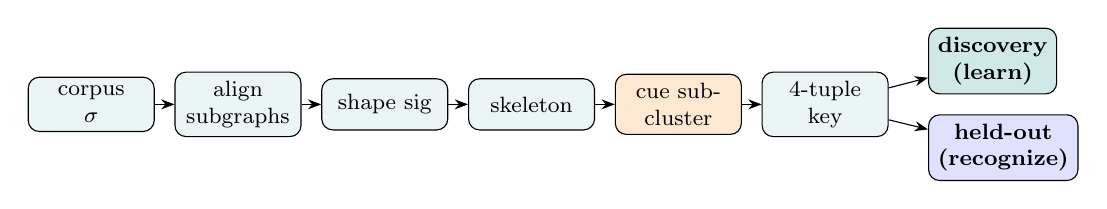
\begin{tikzpicture}[
  box/.style={draw, rounded corners, minimum width=1.6cm, minimum height=0.65cm, font=\footnotesize, align=center, fill=teal!8},
  cue/.style={box, fill=orange!18},
  term/.style={box, minimum width=1.5cm, font=\footnotesize\bfseries},
  node distance=0.25cm,
]
\node[box] (corpus) {corpus\\$\sigma$};
\node[box, right=of corpus] (align) {align\\subgraphs};
\node[box, right=of align] (shape) {shape sig};
\node[box, right=of shape] (skel) {skeleton};
\node[cue, right=of skel] (cue) {cue sub-\\cluster};
\node[box, right=of cue] (route) {4-tuple\\key};
\node[term, right=0.5cm of route, yshift=0.55cm, fill=teal!18] (disc) {discovery\\(learn)};
\node[term, right=0.5cm of route, yshift=-0.55cm, fill=blue!12] (held) {held-out\\(recognize)};
\draw[-Stealth] (corpus) -- (align);
\draw[-Stealth] (align) -- (shape);
\draw[-Stealth] (shape) -- (skel);
\draw[-Stealth] (skel) -- (cue);
\draw[-Stealth] (cue) -- (route);
\draw[-Stealth] (route) -- (disc);
\draw[-Stealth] (route) -- (held);
\end{tikzpicture}
\caption{Structure discovery and cue emergence pipeline. Repeated subgraphs
are aligned and indexed by a discrete shape signature; closed-class cue
tokens are separated from open-class content by sustainable
sub-clustering, yielding a 4-tuple routing key (shape, arity, abstract
signature, cue signature) that routes a sample to discovery (learn) or
held-out recognition (recognize). Cue emergence at the scale required for
end-to-end validation needs $n \geq 300$, currently beyond the
performance envelope (Section~\ref{sec:lim-perf}).}
\label{fig:discovery}
\end{figure}

\subsection{Emergent Correspondence and Sentence Assembly}
\label{sec:mech-corr}
The capstone language mechanism is sentence assembly, and it composes
two independently gated activations. \emph{Structure activation} turns
on a cue position: a skeleton slot whose filler is a closed-class cue
token emits that token directly, so function words (the copula, the
causative) appear at their structural positions rather than being
selected by content. \emph{Abstraction activation} constrains a content
slot: the admissible fillers for a content position are restricted to
tokens that fall under the IS\_A least-common-ancestor class computed
for that slot, so a slot typed by the animal class will not accept a
token that is not a descendant of that class. The two activations are
gated separately and are independently testable, so that structure can
be verified without abstraction and vice versa. Each is implemented
behind default-off gates with unit tests \statusmech.

We are precise about what this assembles. The mechanism produces, at the
level verified today, token-level output---a function word at a cue
position, a class-constrained content token at a content slot---rather
than fluent multi-clause sentences. End-to-end coherent-sentence
generation, in which the two activations compose across a full skeleton
at sentence scale, is deferred behind the performance wall
\statusdeferred.

\subsection{How the Mechanisms Compose}
\label{sec:mech-compose}
These mechanisms are not parallel tracks that compete; they compose in a
fixed priority. A skeleton discovered by alignment
(Section~\ref{sec:mech-discovery}) defines the admissible shape of a
generated utterance---\emph{structure constrains}. Within that shape,
content slots are filled by edge-walking over learned IS\_A/CAUSES edges
(Sections~\ref{sec:mech-arith} and~\ref{sec:mech-corr}), ordered by
tally strength---\emph{content fills}. Sequential order is enforced by
PRECEDES edges, which carry the order in which tokens physically occur
in the corpus (Section~\ref{sec:arch-strata})---\emph{order orders}.
The inverse self-check (Section~\ref{sec:mech-inverse}) sits outside
this priority: it is a consistency check that, if it fires and fails,
vetoes any generation that depends on the pair under test. Because
position is structural and strength is statistical, a strong edge cannot
overpower a skeleton it does not fit: the skeleton is a shape the
generated utterance must take, and a learned edge only selects among
the fillers that shape admits.

\subsection{Memory-Space Side Learning}
Post-weaning acquisition of new facts during interaction is written to
the two-layer memory space rather than to the core concept graph
(Section~\ref{sec:arch-memory}), so conversational learning does not
pollute the trained core. The reading layer holds consolidated
experience shared across sessions; the interaction layer holds
per-conversation ephemeral state; and an item is promoted from the
interaction layer to the reading layer by a usage-ratio gate, so that a
fact must recur before it consolidates \statusmech. This split is what
would later support an online ``learn-by-asking'' capability without
re-training the core: a new fact encountered in conversation would be
written to the interaction layer, consolidated only if it recurred, and
never written to the core graph that the six invariants guard. The
online conversational shell that would exercise this capability is
deferred \statusdeferred.

% ============================================================================
\section{Anti-Theater Engineering Discipline}
\label{sec:antitheater}

\subsection{Stable Is Not Correct}
The central methodological thesis: a mechanism that produces stable
output, passes its tests, and runs deterministically is not thereby
correct. Stability is a property of behavior; correctness is a property
of the relationship to the world. Anti-theater testing validates that the
\emph{criterion} is falsifiable---that the test could in principle
fail---not that the system is semantically correct. The conflation of the
two is the principal failure mode of self-learning systems: a mechanism
wired to produce a passing signal regardless of whether it has learned
anything.

\subsection{Four Mechanism States}
Every mechanism is classified into one of four states, and no claim is
made without stating it: (i) \emph{production-live}, executed on every
run; (ii) \emph{opt-in-gate}, executed only when an explicit gate is
turned on; (iii) \emph{test-only}, present and exercised by tests but
with no production caller; (iv) \emph{dead}, no caller including tests.
The distinction matters: a test-only mechanism is not a system
capability, however sophisticated its implementation. Inline
real-expansion and law-injection are test-only in this architecture: they
never fire on production corpora.

\subsection{Three Weaning Scopes}
Weaning---the withdrawal of the teacher---decomposes into three scopes
that must not be conflated: (i) \emph{pre-weaning}, teacher injection and
replay; (ii) \emph{weaning-verification}, the gated evaluation that the
system produces correct output without the teacher; (iii)
\emph{post-weaning}, autonomous system evolution. A teacher-injected
capability is not a system capability; a post-weaning behavior is not a
verification target. Truth-valued weaning (the decision-layer question
``can the system be weaned?'') is permanently False for the language
domain by design, because it collides with the grounding wall;
statistical-weaning readiness is the strictly weaker, separately defined
question (Section~\ref{sec:mechanisms}).

\subsection{Three-Layer Anti-Theater Harness}
A capability harness evaluates the system across eight dimensions with
three layers of anti-theater checking: (a) \emph{strength delta},
verifying that the learning signal is non-zero (a mechanism with zero
signal has learned nothing); (b) \emph{anchor self-check}, injecting
counter-examples into the corpus so that the main training path itself
produces a failing signal when the criterion is unfalsifiable; (c)
\emph{reverse regression}, injecting fabricated results and verifying
that each dimension fails when it should, with a conservation guard that
prevents a zero-measurement from being scored as a pass. A top-level
flag aborts and elevates the failing dimension. Mutation sensitivity
(simulated monkey-patching) provides a fourth check \statusmech.

\begin{algorithm}[t]
\caption{Three-layer anti-theater capability check}
\label{alg:antitheater}
\begin{algorithmic}[1]
\Require capability dimension $d$, trained system $S$, corpus $\mathcal{C}$
\Ensure pass/fail verdict for $d$
\State \textbf{Layer 1 (strength delta):} measure the learning signal
$\Delta_d$ on $d$; \ \textbf{if} $\Delta_d = 0$ \textbf{then fail}
\Comment{the dimension learned nothing}
\State \textbf{Layer 2 (anchor self-check):} inject counter-examples
into $\mathcal{C}$ and re-train; \ \textbf{if} the criterion still passes
\textbf{then fail} \Comment{criterion is unfalsifiable}
\State \textbf{Layer 3 (reverse regression):} fabricate a passing result
for $d$; \ \textbf{if} the conservation guard scores the zero-measurement
as a pass \textbf{then fail} \Comment{a degenerate pass by silence}
\State \textbf{Layer 4 (mutation sensitivity):} monkey-patch each
mechanism feeding $d$ to a no-op; \ \textbf{if} no dimension fails
\textbf{then fail} \Comment{theater: output is independent of the mechanism}
\State \textbf{return} \textsc{pass} iff all four layers fail to fail
\end{algorithmic}
\end{algorithm}

\subsection{Gate Discipline}
Every new mechanism is admitted behind a default-off gate, so that the
bit-identical baseline (Section~\ref{sec:bitidentical}) is preserved at
every commit; turning a gate on is an explicit, logged behavior change.
This makes the architecture's evolution auditable: any change in output
is attributable to a specific gate transition, never to silent drift.

\subsection{Portability}
This discipline is not a result in itself. It is the supporting practice
that keeps the pure-integer exploration honest: a system this easy to
fool---one whose correctness has no continuous signal to lean on---needs,
more than most, a check that what looks learned really is. The discipline
stays close to the representation that motivates it; whether it ports to
float-based systems is a question we set aside.

% ============================================================================
\section{Honest Limitations}
\label{sec:limitations}

The arithmetic domain is where the construction runs end to end, on a
small corpus whose scope we have stated in the open; the language domain
is where we are still building, and this chapter reports its terrain
honestly. We state what is and is not yet in place, exhaustively;
the four claims below must be qualified whenever they appear, because they
are the points where this line of work is most prone to overstate:

\begin{itemize}[leftmargin=*]
\item \textbf{Fluent dialogue.} The system does not produce fluent
multi-clause sentences. Current output granularity is word- or
phrase-level. The four-layer conversational shell (online ingest and
tokenization, query-to-focus parsing, generation-and-render, and the
read-eval-print loop) is deferred.
\item \textbf{Weaning.} Truth-valued weaning (\textit{can\_ween}) is
permanently False for the language domain (grounding wall) and currently
False globally (the teacher-independence execution condition is not yet
in place). Statistical-weaning readiness is a strictly weaker, separately
defined verdict and is not equivalent to weaning.
\item \textbf{Coherent-sentence generation.} End-to-end generation is
deferred on the performance wall; the mechanism is validated only in
discovery-only mode at scale.
\item \textbf{Language-domain weaning.} Accepted as permanently False at
the decision layer; the statistical-layer path is the contribution, not
decision-layer weaning.
\end{itemize}

\subsection{Two-Axis Diagnosis of the Sentence-Generation Deficit}
\label{sec:lim-twoaxis}

We report this as a negative result: the sentence-generation deficit is
not a single missing piece but a multi-cellular failure we could not
localise to one fixable cell. The red-line list above states \emph{what}
is absent; this subsection states \emph{why}, separating two independent
kinds of gap. A constraint that the system must honour to emit a coherent
sentence can fail in two orthogonal ways, and conflating the two obscures
both:

\begin{itemize}[leftmargin=*]
\item \textbf{Learning-side gap.} The statistical layer has not acquired
the constraint from the training corpus at sufficient strength. The
constraint is genuine, but the edge-count signal that would carry it has
not reached promotion, or has not been written at all.
\item \textbf{Application-side gap.} The constraint has been learned (or
is learnable) but is not brought to bear at generation. This subdivides
into \emph{unimplemented} (no code path exists) and \emph{unwired} (the
path exists but has no production caller, or its alignment key misses the
held-out data).
\end{itemize}

Three constraint classes bear on sentence generation: \emph{order}
(sequential precedence between tokens), \emph{structure} (combinatorial
composition into a skeleton), and \emph{conceptual association} (IS\_A,
CAUSES, REALIZES edges that restrict admissible slot fillers).
Table~\ref{tab:twoaxis} records the current status of each cell. The
deficit is not localized to a single cell: on the structure axis, for
instance, training at $n=300$ produces too few skeletons, and the
held-out probe's variable-length sentences match none of them, so it is
silently vetoed---a learning-side insufficiency compounded by an
application-side mismatch. Lifting the performance wall permits a larger
corpus but does not by itself close either gap.

\begin{table}[t]
\centering
\small
\caption{Two-axis status of the three constraint classes relevant to
coherent-sentence generation. ``Learning'' = status of acquisition from
the training corpus at $n{=}300$; ``Application'' = status of use at
generation. The deficit is multi-cellular: no single cell explains it.}
\label{tab:twoaxis}
\begin{tabular}{@{}p{0.20\linewidth}p{0.30\linewidth}p{0.36\linewidth}@{}}
\toprule
Constraint class & Learning status & Application status \\
\midrule
Order (PRECEDES)            & edges promoted \statusmech       & wired; e2e deferred \statusdeferred \\
Structure (COMPOSES)        & few skeletons learned            & aligned; shape-mismatch \statusdeferred \\
Conceptual (IS\_A/CAUSES/   & boot + tally mechanism \statusmech & cue emergence needs scale \statusdeferred \\
\quad REALIZES)             &                                  & \\
\bottomrule
\end{tabular}
\end{table}

\subsection{Definitive Walls (Permanent)}
The architecture collides with three definitive walls that float-based
systems also cannot cross: (i) the \emph{truth/grounding wall}---definitive
truth values, world reference, and absolute universal extension are
unverifiable; (ii) \emph{physical execution and cross-modal grounding};
(iii) the \emph{semantic cold zone} (zero-co-occurrence pure semantics).
These are not presented as unique failures of this architecture.

\subsection{Engineering Wall and Optimization Path}
\label{sec:lim-perf}
At corpus scale $n=300$, formal training takes approximately 869 seconds,
exceeding the 600-second budget; this blocks end-to-end validation of the
capstone language mechanisms (cue emergence at scale, measured=True, and
coherent-sentence generation). The wall is one of speed, not of
correctness: running at this scale with a relaxed time budget completes,
and the bottleneck is identifiable---repeated full-graph ancestor-map
rebuilds and un-indexed selection scans---rather than architectural.

This is the half of the integers-as-representation guess that was wrong
(Section~\ref{sec:intro-start}): integer computation is exact, but the
integer graph operations it requires are not cheap. We record the
optimization path as future work rather than a limitation in principle.
The profiled targets are concrete: memoizing nearest-ancestor lookups
within a segment, adding a covering index on the abstract-mark table, and
caching selection keys together remove the bulk of the repeated scan
cost; incremental (dirty-flag) ancestor-map updates replace per-segment
full rebuilds. Together these are projected to bring $n=300$ under
budget; sub-budget scaling at larger $n$ would require incremental
dependency-path computation, a deeper restructuring. A longer-term
option is to rewrite the compute-intensive core in a native language
while keeping the integer invariants and the AST audit intact---an
engineering change, not a change to the contract.

\subsection{Mechanisms Present but Not Live}
Several mechanisms are present in the codebase but not live in
production: inline real-expansion and law-injection are test-only (zero
production fire); analytic-priority code (closed-form discovery,
polynomial support) resides in the legacy archive and is not rebuilt;
some property-evaluation paths are structurally non-evaluating. These are
design-complete or test-only, not capabilities.

\subsection{Deferred Mechanisms}
Multimodal modalities (audio, 2D, 3D) have minimal-loop designs deferred
to non-language triggering; a pseudo-continuous measurable framework is
deferred; a rational-vector metric space was considered and rejected on
grounds of training cost without semantic gain. The five-anchor measured
flags (fade-out, floor, and held-out at language scale) are not yet
empirically True at the time of writing.

% ============================================================================
\section{Related Work}
\label{sec:related}

\subsection{Float-Based Learners}
The dominant paradigm---large language models \citep{vaswani2017attention},
graph neural networks \citep{gilmer2017neural}, and reinforcement learners
\citep{mnih2015human}---represents learned state as floating-point
weights optimized by gradient descent, a learning rule whose lineage
traces to backpropagation \citep{rumelhart1986learning} and whose
value-function variants are formalized in the reinforcement-learning
framework \citep{sutton2018rl}. Our architecture differs in kind:
state is integer edges, learning is statistical reinforcement, and the
reproducibility property is exact rather than approximate. We do not
claim superiority on tasks where float-based systems excel; we claim a
different and complementary set of guarantees. Concretely, the three
defects named in Section~\ref{sec:intro-motivation} are exactly the ones
a large model cannot self-certify: it cannot point to the edge behind a
given fact, cannot reproduce byte-for-byte across machines, and cannot
mechanically separate what it was taught from what it inferred. A
pure-integer core can supply all three as checked properties, so the
complementary role we can see is not ``another learner that competes on
benchmarks'' but an auditable substrate---a learned store whose facts
are individually addressable and whose changes are attributable to a
named transition. Whether such a substrate can carry enough learned
content to be useful alongside a large model is the open question this
paper does not settle; we claim only that the guarantees are real and
unavailable to a float representation, not that they are sufficient for
any task in particular.

\subsection{Symbolic and Neuro-Symbolic Systems}
Symbolic AI \citep{russell2010artificial} represents knowledge as discrete
structures but typically relies on external inference engines and lacks
the monotone statistical learning dynamics studied here. Inductive logic
programming \citep{muggleton1991ilp} learns Horn-clause rules from
examples---a symbolic-learning tradition we share in spirit, but differ
from in replacing logical unification with integer edge-count
reinforcement. Neuro-symbolic systems \citep{garcez2020neurosymbolic}
combine neural perception with symbolic reasoning but inherit
floating-point nondeterminism on the neural side. This architecture is
symbolic throughout, with learning expressed as integer edge-count
reinforcement.

Lexical resources such as WordNet \citep{miller1995wordnet} and
corpus-based hyponym acquisition \citep{hearst1992hyponyms} supply the
kind of IS\_A / hypernym structure that our system learns from
co-occurrence rather than imports as a prefabricated table; the
closed-class acquisition of function-word and role signals from exposure
(Section~\ref{sec:arch-learning}) is the structural analogue of Hearst
pattern mining, performed online as learned edges rather than as offline
lexicon construction.

\subsection{Reproducible Machine Learning}
The reproducibility crisis in machine learning
\citep{pineau2021improving} has motivated deterministic-training
protocols, fixed seeds, and benchmark snapshots.
These efforts operate within the float representation and therefore
achieve approximate reproducibility; the bit-identical guarantee here is
exact and follows from the representation, not from a protocol layered on
top of it.

\subsection{Program Synthesis and Self-Proof}
Program synthesis \citep{gulwani2017synthesis} constructs programs from
specifications, typically by search over a typed grammar with external
verification. Our arithmetic self-proof (Section~\ref{sec:mechanisms})
inverts the usual relation: the system generates an answer and then
\emph{re-derives} it as its own correctness check, with a mismatch
yielding zero reward. The verification is internal and integer-exact,
not supplied by an external solver.

\smallskip\noindent\textit{Terminology note.} Where adjacent literature
uses differential-geometry terms (curvature, holonomy, fibre bundle) for
related structural concepts, we adopt the integer-graph vocabulary of
Section~\ref{sec:mechanisms} and Appendix~\ref{app:terms} for
freedom-to-operate reasons; the mapping is given in
Table~\ref{tab:terms}.

% ============================================================================
\section{Conclusion}
\label{sec:conclusion}

We set out to ask whether an intelligent system can be built entirely
on integers. The project that asked it began, in honesty, from a smaller
and less dignified place: a frustration with assistants that forget, on
a machine that could not host a large model, and a guess that integers
might cost less than floats. The guess about cost was wrong, as we have
said. What proved worth keeping was the representation the guess left
behind---a learned state made of discrete, addressable integer
structures, auditable one fact at a time and reproducible across
machines.

We have not answered the question in full, but we report how far the
construction goes. The core is strictly pure-integer and runs; the six
invariants hold it together and admit no quiet exception; and in the
arithmetic domain the construction runs end to end: it compiles a
symbolic specification, executes it on the integer core, self-checks by
recomputation, and passes a six-gate readiness check that we define
narrowly and falsifiably. We have been precise that this is a mechanism
demonstration on a small, hand-shaped corpus, not acquired arithmetic in
a strong sense, and that genuine generalisation is the work still ahead.
The approach has not yet been shown to reach a real verdict in any
domain. What we can say is that the construction holds together, runs,
and makes claims that can actually be checked.

We are aware of the obvious objection: that a construction celebrated for
its honesty, with no capability to match, is a cage without an animal in
it. We do not dispute the premise---the system has not been shown to
produce competitive intelligent behaviour, and this paper does not claim
it will. What we do claim is that the honesty is itself a result, not an
absence. In a setting where a learned system cannot be inspected,
reproduced, or told apart from what it was taught, the ability to do all
three is a property that has to be built and checked; it does not come
for free with any representation. Whether the representation that admits
this honesty can be made to carry enough learned content to be useful is
the question the rest of the construction is there to answer. We report
the construction because it is what we have, and because a claim that can
be checked is, for this architecture, the only kind worth making.

Much remains. The language domain---the next thing we are trying to
build on the same construction---has its mechanisms in place but has not
yet reached the same verdict, held back by an engineering wall rather
than an architectural one. Coherent sentence generation, the
conversational shell, the local-memory layer that motivated this work in
the first place, and readiness at language scale are open. Each is a
gated, auditable step on the same construction, not a change to the
contract. We report these gaps plainly because the value of the
approach, if it has any, is in being a system whose claims can actually
be checked---and a claim that cannot be checked is, for this
construction, no claim at all.

% ============================================================================
\appendix

\section{Terminology Decoupling Table}
\label{app:terms}

For freedom-to-operate reasons the body of this paper uses an
integer-graph vocabulary in place of differential-geometry terms that
appear in some adjacent literature. Table~\ref{tab:terms} maps the
terms; the left column is used only when explicitly citing prior work.

\begin{table}[h]
\centering
\small
\caption{Terminology mapping. Body text uses the right column.}
\label{tab:terms}
\begin{tabular}{@{}p{0.35\linewidth}p{0.50\linewidth}@{}}
\toprule
Term avoided in body & Term used instead \\
\midrule
curvature                  & loop-closure defect \\
holonomy                   & cycle-inconsistency \\
fibre bundle / fiber bundle & integer graph / structural sheet \\
\bottomrule
\end{tabular}
\end{table}

\section{Reproducibility Kit}
\label{app:repro}

To reproduce bit-identical output: (i) set \texttt{PYTHONHASHSEED=0};
(ii) set the hot-zone environment variables that bound the activation
search (\texttt{DAG\_PATH\_REACHABLE\_SCOPE\_MODE=1},
\texttt{DAG\_HOPS=2}, \texttt{STRUCT\_REF\_CONTENT\_HASH\_MODE=1});
(iii) keep all gates at their default (off) configuration;
(iv) run the bit-identical test suite, which compares terminal hashes
across two passes under the same seed and asserts equality. Turning a
gate on is a logged behavior change that remains deterministic within
the chosen configuration but is not bit-identical to the gate-off
baseline.

The reference implementation is the \texttt{pure\_integer\_ai} package
(named for its core invariant, not as a trademark). The reproduction
commands are:
\begin{itemize}[leftmargin=*]
\item \texttt{PYTHONHASHSEED=0 python -m pytest tests/ -q} --- the full
test suite (2376 tests at the time of writing), including the
bit-identical two-pass assertion and the FC-family boundary tests.
\item \texttt{python -m pure\_integer\_ai.crosscut.guards.lint} --- the
three static lints (no-floating-point, no forbidden
\texttt{time}/\texttt{datetime}/\texttt{random} calls, downward-only
import direction) that enforce the core invariants at the AST level.
\end{itemize}
The gate-off configuration is the continuous-integration baseline:
every commit is required to be bit-identical to its predecessor unless a
gate is explicitly toggled, so the architecture's evolution is an
auditable sequence of named transitions rather than silent drift.

\bibliographystyle{plainnat}
\bibliography{refs}

\end{document}
